% -*- latex -*-
%%%%%%%%%%%%%%%%%%%%%%%%%%%%%%%%%%%%%%%%%%%%%%%%%%%%%%%%%%%%%%%%
%%%%%%%%%%%%%%%%%%%%%%%%%%%%%%%%%%%%%%%%%%%%%%%%%%%%%%%%%%%%%%%%
%%%%
%%%% This text file is part of the source of 
%%%% `Parallel Programming in MPI and OpenMP'
%%%% by Victor Eijkhout, copyright 2012-2022
%%%%
%%%% petsc-objects.tex : petsc tangible-ish objects
%%%%
%%%%%%%%%%%%%%%%%%%%%%%%%%%%%%%%%%%%%%%%%%%%%%%%%%%%%%%%%%%%%%%%
%%%%%%%%%%%%%%%%%%%%%%%%%%%%%%%%%%%%%%%%%%%%%%%%%%%%%%%%%%%%%%%%

\Level 0 {Distributed objects}

PETSc is based on the \ac{SPMD} model, and all its objects act like
they exist in parallel, spread out over all the processes.  Therefore,
prior to discussing specific objects in detail, we briefly discuss how
PETSc treats distributed objects.

For a matrix or vector you need to specify the size. This can be done two ways:
\begin{itemize}
\item you specify the global size and PETSc distributes the object over the processes, or
\item you specify on each process the local size
\end{itemize}
If you specify both the global size and the local sizes, PETSc will check for consistency.

For example, if you have a vector of $N$ components, or a matrix of $N$
rows, and you have $P$ processes, each process will receive $N/P$
components or rows if $P$ divides evenly in~$N$. If $P$ does not divide
evenly, the excess is spread over the processes.

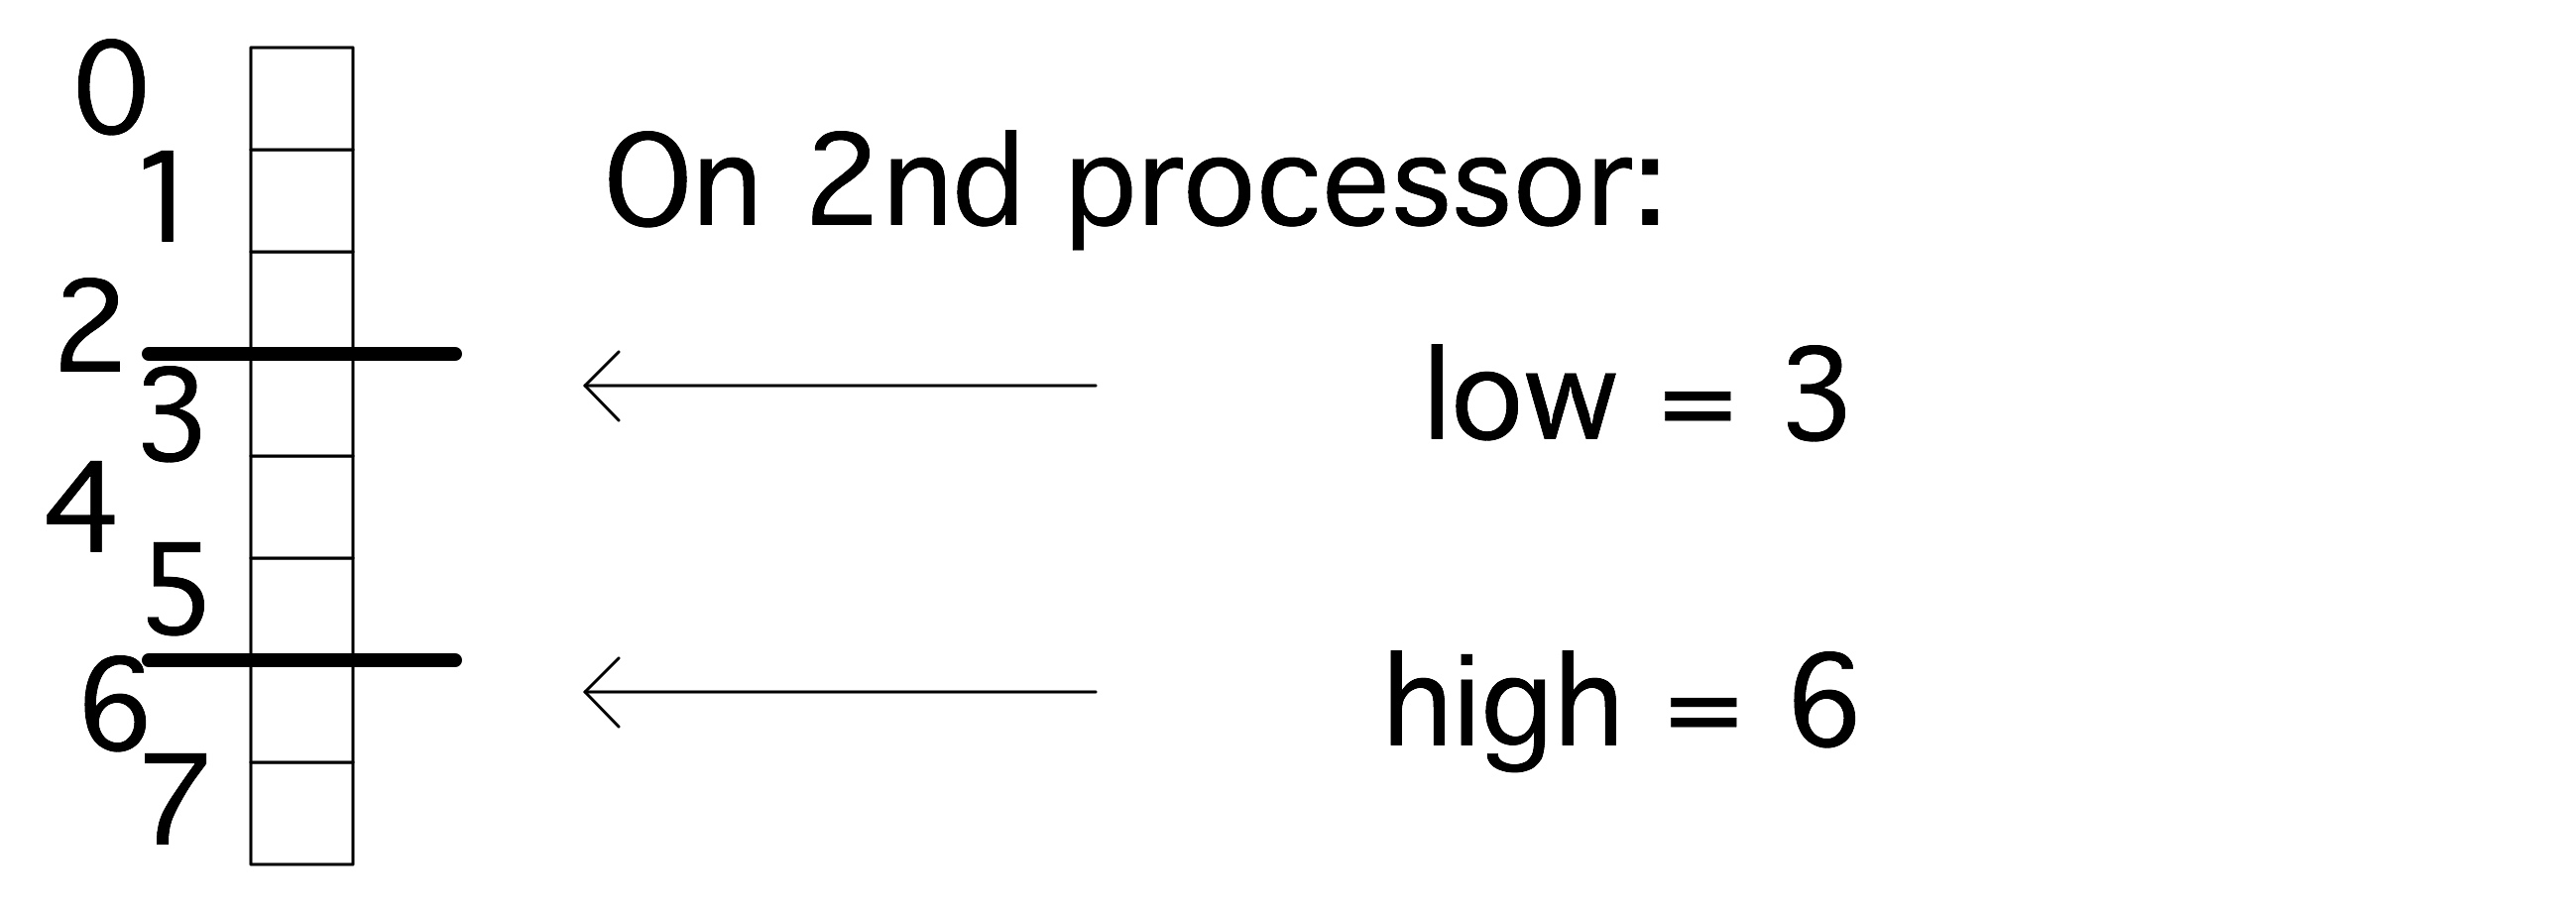
\includegraphics[scale=.1]{veclayout}

The way the distribution is done is by contiguous blocks: with 10
processes and 1000 components in a vector, process 0 gets the range
$0\cdots99$, process 1 gets $1\cdots199$, et cetera. This simple scheme suffices for
many cases, but PETSc has facilities for more sophisticated load
balancing.

\Level 1 {Support for distributions}

Once an object has been created and distributed, you do not need to
remember the size or the distribution yourself: you can query these
with calls such as \clstinline{VecGetSize},
\clstinline{VecGetLocalSize}.

The
corresponding matrix routines \clstinline{MatGetSize},
\clstinline{MatGetLocalSize} give both information for the
distributions in $i$ and~$j$ direction, which can be
independent. Since a matrix is distributed by rows,
\clstinline{MatGetOwnershipRange} only gives a row range.

\cverbatimsnippet[examples/petsc/c/split.c]{splitownersnip}

While PETSc objects are implemented using local memory on each
process, conceptually they act like global objects, with a global
indexing scheme. Thus, each process can query which elements out of
the global object are stored locally.
For vectors, the relevant routine is \clstinline{VecGetOwnershipRange},
which returns two parameters, \clstinline{low} and~\clstinline{high},
respectively the first element index stored, and
one-more-than-the-last index stored.

This gives the idiom:
\begin{lstlisting}
VecGetOwnershipRange(myvector,&low,&high);
for (int myidx=low; myidx<high; myidx++)
  // do something at index myidx
\end{lstlisting}

These conversions between local and global size can also be done
explicitly, using the \indexpetscref{PetscSplitOwnership} routine.
This routine takes two parameter, for the local and global size, and
whichever one is initialized to \indexpetscshow{PETSC_DECIDE} gets
computed from the other.

\Level 0 {Scalars}
\label{sec:petsc-scalar}

Unlike programming languages that explicitly distinguish between
single and double precision numbers, PETSc has only a single scalar
type: \indexpetscdef{PetscScalar}. The precision of this is determined
at installation time. In fact, a \clstinline{PetscScalar} can even be a
complex number if the installation specified that the scalar type is
complex.

Even in applications that use complex numbers there can be quantities
that are real: for instance, the norm of a complex vector is a real
number. For that reason, PETSc also has the type
\indexpetscdef{PetscReal}. There is also an explicit \indexpetscdef{PetscComplex}.

Furthermore, there is
\begin{lstlisting}
#define PETSC_BINARY_INT_SIZE    (32/8)
#define PETSC_BINARY_FLOAT_SIZE  (32/8)
#define PETSC_BINARY_CHAR_SIZE   (8/8)
#define PETSC_BINARY_SHORT_SIZE  (16/8)
#define PETSC_BINARY_DOUBLE_SIZE (64/8)
#define PETSC_BINARY_SCALAR_SIZE sizeof(PetscScalar)  
\end{lstlisting}

\Level 1 {Integers}

Integers in PETSc are likewise of a size determined at installation
time: \indexpetscdef{PetscInt} can be 32 or 64 bits.
The latter possibility is useful for indexing into large vectors and matrices.
Furthermore,
there is a \indexpetscshow{PetscErrorCode} type for catching the return
code of PETSc routines; see section~\ref{sec:petsc-error}.

For compatibility with other packages there are two more integer types:
\index{PETSc!interoperability with MPI}%
\index{PETSc!interoperability with BLAS}%
\begin{itemize}
\item \indexpetscdef{PetscBLASInt} is the integer type used by the
  \indexac{BLAS}~/ \indexac{LAPACK} library. This is 32-bits if the
  \indexpetscshow{-download-blas-lapack} option is used, but it can be 64-bit if
  \indexterm{MKL} is used.
  The routine \indexpetscdef{PetscBLASIntCast} casts a
  \indexpetscshow{PetscInt} to \indexpetscshow{PetscBLASInt}, or returns
  \indexpetscshow{PETSC_ERR_ARG_OUTOFRANGE} if it is too large.
\item \indexpetscdef{PetscMPIInt} is the integer type of the MPI library, which is
  always 32-bits.
  The routine \indexpetscdef{PetscMPIIntCast} casts a
  \indexpetscshow{PetscInt} to \indexpetscshow{PetscMPIInt}, or returns
  \indexpetscshow{PETSC_ERR_ARG_OUTOFRANGE} if it is too large.
\end{itemize}
Many external packages do not support 64-bit integers.

\Level 1 {Complex}

Numbers of type \indexpetscshow{PetscComplex} have a precision
matching \indexpetscshow{PetscReal}.

Form a complex number using \indexpetscdef{PETSC_i}:
\begin{lstlisting}
PetscComplex x = 1.0 + 2.0 * PETSC_i;
\end{lstlisting}

The real and imaginary part can be extract with the functions
\indexpetscdef{PetscRealPart} and \indexpetscdef{PetscImaginaryPart}
which return a \indexpetscshow{PetscReal}.

There are also routines \indexpetscdef{VecRealPart}
and \indexpetscdef{VecImaginaryPart} that replace a vector
with its real or imaginary part respectively.
Likewise \indexpetscdef{MatRealPart} and \indexpetscdef{MatImaginaryPart}.

\Level 1 {MPI Scalars}

For MPI calls, \indexpetscdef{MPIU_REAL} is the MPI type
corresponding to the current \indexpetscshow{PetscReal}.

For MPI calls, \indexpetscdef{MPIU_SCALAR} is the MPI type
corresponding to the current \indexpetscshow{PetscScalar}.

For MPI calls, \indexpetscdef{MPIU_COMPLEX} is the MPI type
corresponding to the current \indexpetscshow{PetscComplex}.

\Level 1 {Booleans}

There is a \indexpetscdef{PetscBool} datatype
with values \indexpetscdef{PETSC_TRUE} and \indexpetscdef{PETSC_FALSE}.

\Level 0 {Vec: Vectors}

Vectors are objects with a linear index. The elements of a vector are
floating point numbers or complex numbers (see
section~\ref{sec:petsc-scalar}), but not integers: for that see
section~\ref{sec:petsc-is}.

\Level 1 {Vector construction}

Constructing a vector takes a number of steps. First of all, the
vector object needs
to be created on a communicator with
%
\indexpetscref{VecCreate}

\begin{pythonnote}{Vector creation}
  In python, \plstinline{PETSc.Vec()} creates an object with null handle, so a
  subsequent \plstinline{create()} call is needed.
  %
  In C and Fortran, the vector type is a keyword; in Python it is a
  member of \n{PETSc.Vec.Type}.
  %
  \pverbatimsnippet{pyveccreate}
\end{pythonnote}

The corresponding routine \indexpetscref{VecDestroy} deallocates data and zeros
the pointer.
(This and all other Destroy routines are collective because of underlying
MPI technicalities.)

The vector type needs to be set with \indexpetscref{VecSetType}.

The most common vector types are:
\begin{itemize}
\item \indexpetscshow{VECSEQ} for sequential vectors, that is, living on a single process;
  This is typically created on the \indexmpishow{MPI_COMM_SELF} or
  \indexpetscshow{PETSC_COMM_SELF} communicator.
\item \indexpetscshow{VECMPI} for a vector distributed over the communicator.
  This is typically created on the \indexmpishow{MPI_COMM_WORLD} or
  \indexpetscshow{PETSC_COMM_WORLD} communicator, or one derived from it.
\item \indexpetscshow{VECSTANDARD} is \indexpetscshow{VECSEQ} when used on a single process,
  or \indexpetscshow{VECMPI} on multiple.
\end{itemize}

You may wonder why these types exist: you could have just one type,
which would be as parallel as possible.
The reason is that in a parallel run you may occasionally
have a separate linear system on each process, which
would require a sequential vector (and matrix) on each process,
not part of a larger linear system.

Once you have created one vector, you can make more like it by
\indexpetscdef{VecDuplicate},
\begin{lstlisting}
VecDuplicate(Vec old,Vec *new);
\end{lstlisting}
or \indexpetscdef{VecDuplicateVecs}
\begin{lstlisting}
VecDuplicateVecs(Vec old,PetscInt n,Vec **new);
\end{lstlisting}
for multiple vectors.
For the latter, there is a joint destroy call
\indexpetscdef{VecDestroyVecs}:
\begin{lstlisting}
VecDestroyVecs(PetscInt n,Vec **vecs);
\end{lstlisting}
(which is different in Fortran).

\Level 1 {Vector layout}

Next in the creation process the vector size is set with \indexpetscref{VecSetSizes}.
Since a
vector is typically distributed, this involves the global size and the
sizes on the processors. Setting both is redundant, so it is possible
to specify one and let the other be computed by the library. This is
indicated by setting it to \indexpetscdef{PETSC_DECIDE}.

\begin{pythonnote}{Vector size}
  Use \plstinline{PETSc.DECIDE} for the parameter not specified:
  \pverbatimsnippet{pyvecsize}
\end{pythonnote}

The size is queried with \indexpetscref{VecGetSize} for the global size
and \indexpetscxref{VecGetLocalSize}{VecGetSize} for the local size.

Each processor gets a contiguous part of the vector. Use
\indexpetscref{VecGetOwnershipRange} to query the first index on this
process, and the first one of the next process.

In general it is best to let PETSc take care of memory management of
matrix and vector objects, including allocating and freeing the memory.
However, in cases where PETSc interfaces to other applications it maybe desirable
to create a \clstinline{Vec} object from an already
allocated array: \indexpetscdef{VecCreateSeqWithArray} and
\indexpetscdef{VecCreateMPIWithArray}.
\begin{lstlisting}
VecCreateSeqWithArray
   (MPI_Comm comm,PetscInt bs,
    PetscInt n,PetscScalar *array,Vec *V);
VecCreateMPIWithArray
   (MPI_Comm comm,PetscInt bs,
    PetscInt n,PetscInt N,PetscScalar *array,Vec *vv);  
\end{lstlisting}

As you will see in section~\ref{sec:petscmat-create},
you can also create vectors based on the layout of a matrix,
using \indexpetscshow{MatCreateVecs}.

\Level 1 {Vector operations}

There are many routines operating on vectors that you need
to write scientific applications. Examples are: norms, vector addition
(including \ac{BLAS}-type `AXPY' routines: \indexpetscref{VecAXPY}),
pointwise scaling, inner products.
A~large number of such operations are available in PETSc through
single function calls to {VecXYZ} routines.

For debugging purpoases,
the \indexpetscref{VecView} routine can be used to display vectors on screen as
ascii output,
%
\cverbatimsnippet[examples/petsc/c/fftsine.c]{vecviewbeforeafter}
%
but the routine call also use more general \clstinline{PetscViewer} objects, for
instance to dump a vector to file.

Here are a couple of representative vector routines:
\begin{lstlisting}
PetscReal lambda;
ierr = VecNorm(y,NORM_2,&lambda); CHKERRQ(ierr);
ierr = VecScale(y,1./lambda); CHKERRQ(ierr);  
\end{lstlisting}

\begin{exercise}
  Create a vector where the values are a single sine wave.
  using \indexpetscshow{VecGetSize}, \indexpetscshow{VecGetLocalSize},
  \indexpetscshow{VecGetOwnershipRange}.
  Quick visual inspection:
\begin{verbatim}
ibrun vec -n 12 -vec_view
\end{verbatim}
  \skeleton{vec}
\end{exercise}

\begin{exercise}
Use the routines \indexpetscref{VecDot}, \indexpetscref{VecScale}
and \indexpetscref{VecNorm} to compute the inner product of vectors
\n{x,y}, scale the vector~\n{x}, and check its norm:
\[
\begin{array}{l}
p \leftarrow x^ty\\
x \leftarrow x/p\\
n \leftarrow \|x\|_2\\
\end{array}
\]
\end{exercise}

\begin{pythonnote}{Vector operations}
  The plus operator is overloaded so that
  \begin{lstlisting}
    x+y
  \end{lstlisting}
  is defined.
  \begin{lstlisting}
    x.sum() # max,min,....
    x.dot(y)
    x.norm(PETSc.NormType.NORM_INFINITY)
  \end{lstlisting}
\end{pythonnote}

\Level 2 {Split collectives}

MPI is capable (in principle) of `overlapping computation and communication',
or \indextermbus{latency}{hiding}. PETSc supports this
by splitting norms and inner products into two phases.
\begin{itemize}
\item Start inner product~/ norm with \indexpetscdef{VecDotBegin}~/
  \indexpetscdef{VecNormBegin};
\item Conclude inner product~/ norm with \indexpetscdef{VecDotEnd}~/
  \indexpetscdef{VecNormEnd};
\end{itemize}
Even if you achieve no overlap, it is possible to use these calls to
combine a number of `collectives': do the \n{Begin} calls of one inner
product and one norm; then do (in the same sequence) the \n{End} calls.
This means that only a single reduction is performed on a two-word
package, rather than two separate reductions on a single word.

\Level 1 {Vector elements}

Setting elements of a traditional array is simple. Setting elements of
a distributed array is harder.
First of all, \indexpetscdef{VecSet} sets the vector to a constant value:
\begin{lstlisting}
ierr = VecSet(x,1.); CHKERRQ(ierr);  
\end{lstlisting}

In the general case, setting elements in a PETSc vector is done
through a
function \indexpetscref{VecSetValue} for setting elements that uses global numbering; any
process can set any elements in the vector.
%
There is also a routine \indexpetscref{VecSetValues} for setting
multiple elements. This is mostly useful for setting dense subblocks
of a block matrix.

We illustrate both routines by setting a single element with \indexpetscshow{VecSetValue},
and two elements with \indexpetscshow{VecSetValues}. In the latter case
we need an array of length two for both the indices and values. The indices need
not be successive.

\lstset{language=C}
\begin{lstlisting}
i = 1; v = 3.14;
VecSetValue(x,i,v,INSERT_VALUES);
ii[0] = 1; ii[1] = 2; vv[0] = 2.7; vv[1] = 3.1;
VecSetValues(x,2,ii,vv,INSERT_VALUES);
\end{lstlisting}

\begin{fortrannote}{Setting values}
  The value/values routines work the same way in Fortran.
  Note that despite type checking, using the `values' routine
  and passing scalars, is allowed:
  %
  \fverbatimsnippet{valuevaluesf}
\end{fortrannote}

\begin{pythonnote}{Setting vector values}
  Single element:
  \pverbatimsnippet{pyvecval}
  Multiple elements:
  \pverbatimsnippet{pyvecvals}
\end{pythonnote}

Using \clstinline{VecSetValue} for specifying a local vector element
corresponds to simple insertion in the local array. However,
an element that belongs to another process needs to be
transferred. This done in two calls: \indexpetscref{VecAssemblyBegin}
and \indexpetscshow{VecAssemblyEnd}.

\fverbatimsnippet[examples/petsc/f/vecset.F90]{vecsetfrom0}

(If you know the MPI library, you'll recognize that the first call corresponds to
posting nonblocking send and receive calls; the second then contains
the wait calls. Thus, the existence of these separate calls make
\indextermbus{latency}{hiding} possible.)

\begin{lstlisting}
VecAssemblyBegin(myvec);
// do work that does not need the vector myvec
VecAssemblyEnd(myvec);
\end{lstlisting}

Elements can either be inserted
with \indexpetscshow{INSERT_VALUES},
or added with \indexpetscshow{ADD_VALUES} in the
\indexpetscshow{VecSetValue}~/ \indexpetscshow{VecSetValues} call.
You can not immediately mix these modes; to do so you need to call
\indexpetscshow{VecAssemblyBegin}~/ \indexpetscshow{VecAssemblyEnd}
in between add/insert phases.

\Level 2 {Explicit element access}

Since the vector routines cover a large repertoire of operations, you
hardly ever need to access the actual elements. Should you still need
those elements, you can use \indexpetscref{VecGetArray} for general
access or \indexpetscxref{VecGetArrayRead}{VecGetArray} for read-only.

PETSc insists that you properly release this pointer again with
\indexpetscref{VecRestoreArray} or
\indexpetscxref{VecRestoreArrayRead}{VecRestoreArray}.

In the following example, a vector is scaled through direct array access.
Note the differing calls for the source and target vector,
and note the \lstinline{const} qualifier on the source array:
%
\cverbatimsnippet{vecgetarray}

This example also uses \indexpetscshow{VecGetLocalSize}
to determine the size of the data accessed.
Even running in a distributed context you can only get the array
of local elements.
Accessing the elements from another process
requires explicit communication; see section~\ref{sec:petsc-vs}.

There are some variants to the \clstinline{VecGetArray} operation:
\begin{itemize}
\item \indexpetscxref{VecReplaceArray}{VecPlaceArray} frees the memory of the
  \clstinline{Vec} object, and replaces it with a different array. That
  latter array needs to be allocated with
  \indexpetscshow{PetscMalloc}.
\item \indexpetscref{VecPlaceArray} also installs a new array in the
  vector, but it keeps the original array; this can be restored with
  \indexpetscdef{VecResetArray}.
\end{itemize}

Putting the array of one vector into another has a common application,
where you have a distributed vector, but want to apply PETSc operations
to its local section as if it were a sequential vector. In that case
you would create a sequential vector, and
\indexpetscshow{VecPlaceArray} the contents of the distributed vector
into it.

\begin{fortrannote}{F90 array access through pointer}
  There are routines such as \indexpetscdef{VecGetArrayF90}
  (with corresponding \indexpetscdef{VecRestoreArrayF90})
  that
  return a (Fortran) pointer to a one-dimensional array.
  %
  \fverbatimsnippet[examples/petsc/f/vecset.F90]{vecinspect90}
  \fverbatimsnippet[examples/petsc/f08/vecarray.F90]{pfvecgetarray}
\end{fortrannote}

\begin{pythonnote}{Vector access}
  \begin{lstlisting}
    x.getArray()
    x.getValues(3)
    x.getValues([1, 2])
  \end{lstlisting}
\end{pythonnote}

\Level 1 {File I/O}
\label{sec:vecviewload}

As mentioned above, \indexpetscshow{VecView} can be used for
displaying a vector on the terminal screen.
However, viewers are actually much more general.
As explained in section~\ref{sec:petsc-view},
they can also be used to export vector data, for instance to file.

The converse operation, to load a vector that was exported in this manner,
is \indexpetscdef{VecLoad}.

Since these operations are each other's inverses,
usually you don't need to know the file format.
But just in case:
\begin{lstlisting}
PetscInt    VEC_FILE_CLASSID
PetscInt    number of rows
PetscScalar *values of all entries
\end{lstlisting}
That is, the file starts with a magic number, then the number of vector elements,
and subsequently all scalar values.

\Level 0 {Mat: Matrices}

PETSc matrices come in a number of types, sparse and dense being the
most important ones. Another possibility is to have the matrix in
operation form, where only the action $y\leftarrow Ax$ is defined.

\Level 1 {Matrix creation}
\label{sec:petscmat-create}

Creating a matrix also starts by specifying a communicator on which
the matrix lives collectively:
%
\indexpetscref{MatCreate}

Set the matrix type with \indexpetscref{MatSetType}.  The main choices
are between sequential versus distributed and dense versus sparse,
giving types: \indexpetscshow{MATMPIDENSE}, \indexpetscshow{MATMPIAIJ},
\indexpetscshow{MATSEQDENSE}, \indexpetscshow{MATSEQAIJ}.

Distributed matrices are partitioned by block rows: each process
stores a \indexterm{block row}, that is, a contiguous set of matrix
rows. It stores all elements in that block row.
%
\begin{figure}[ht]
  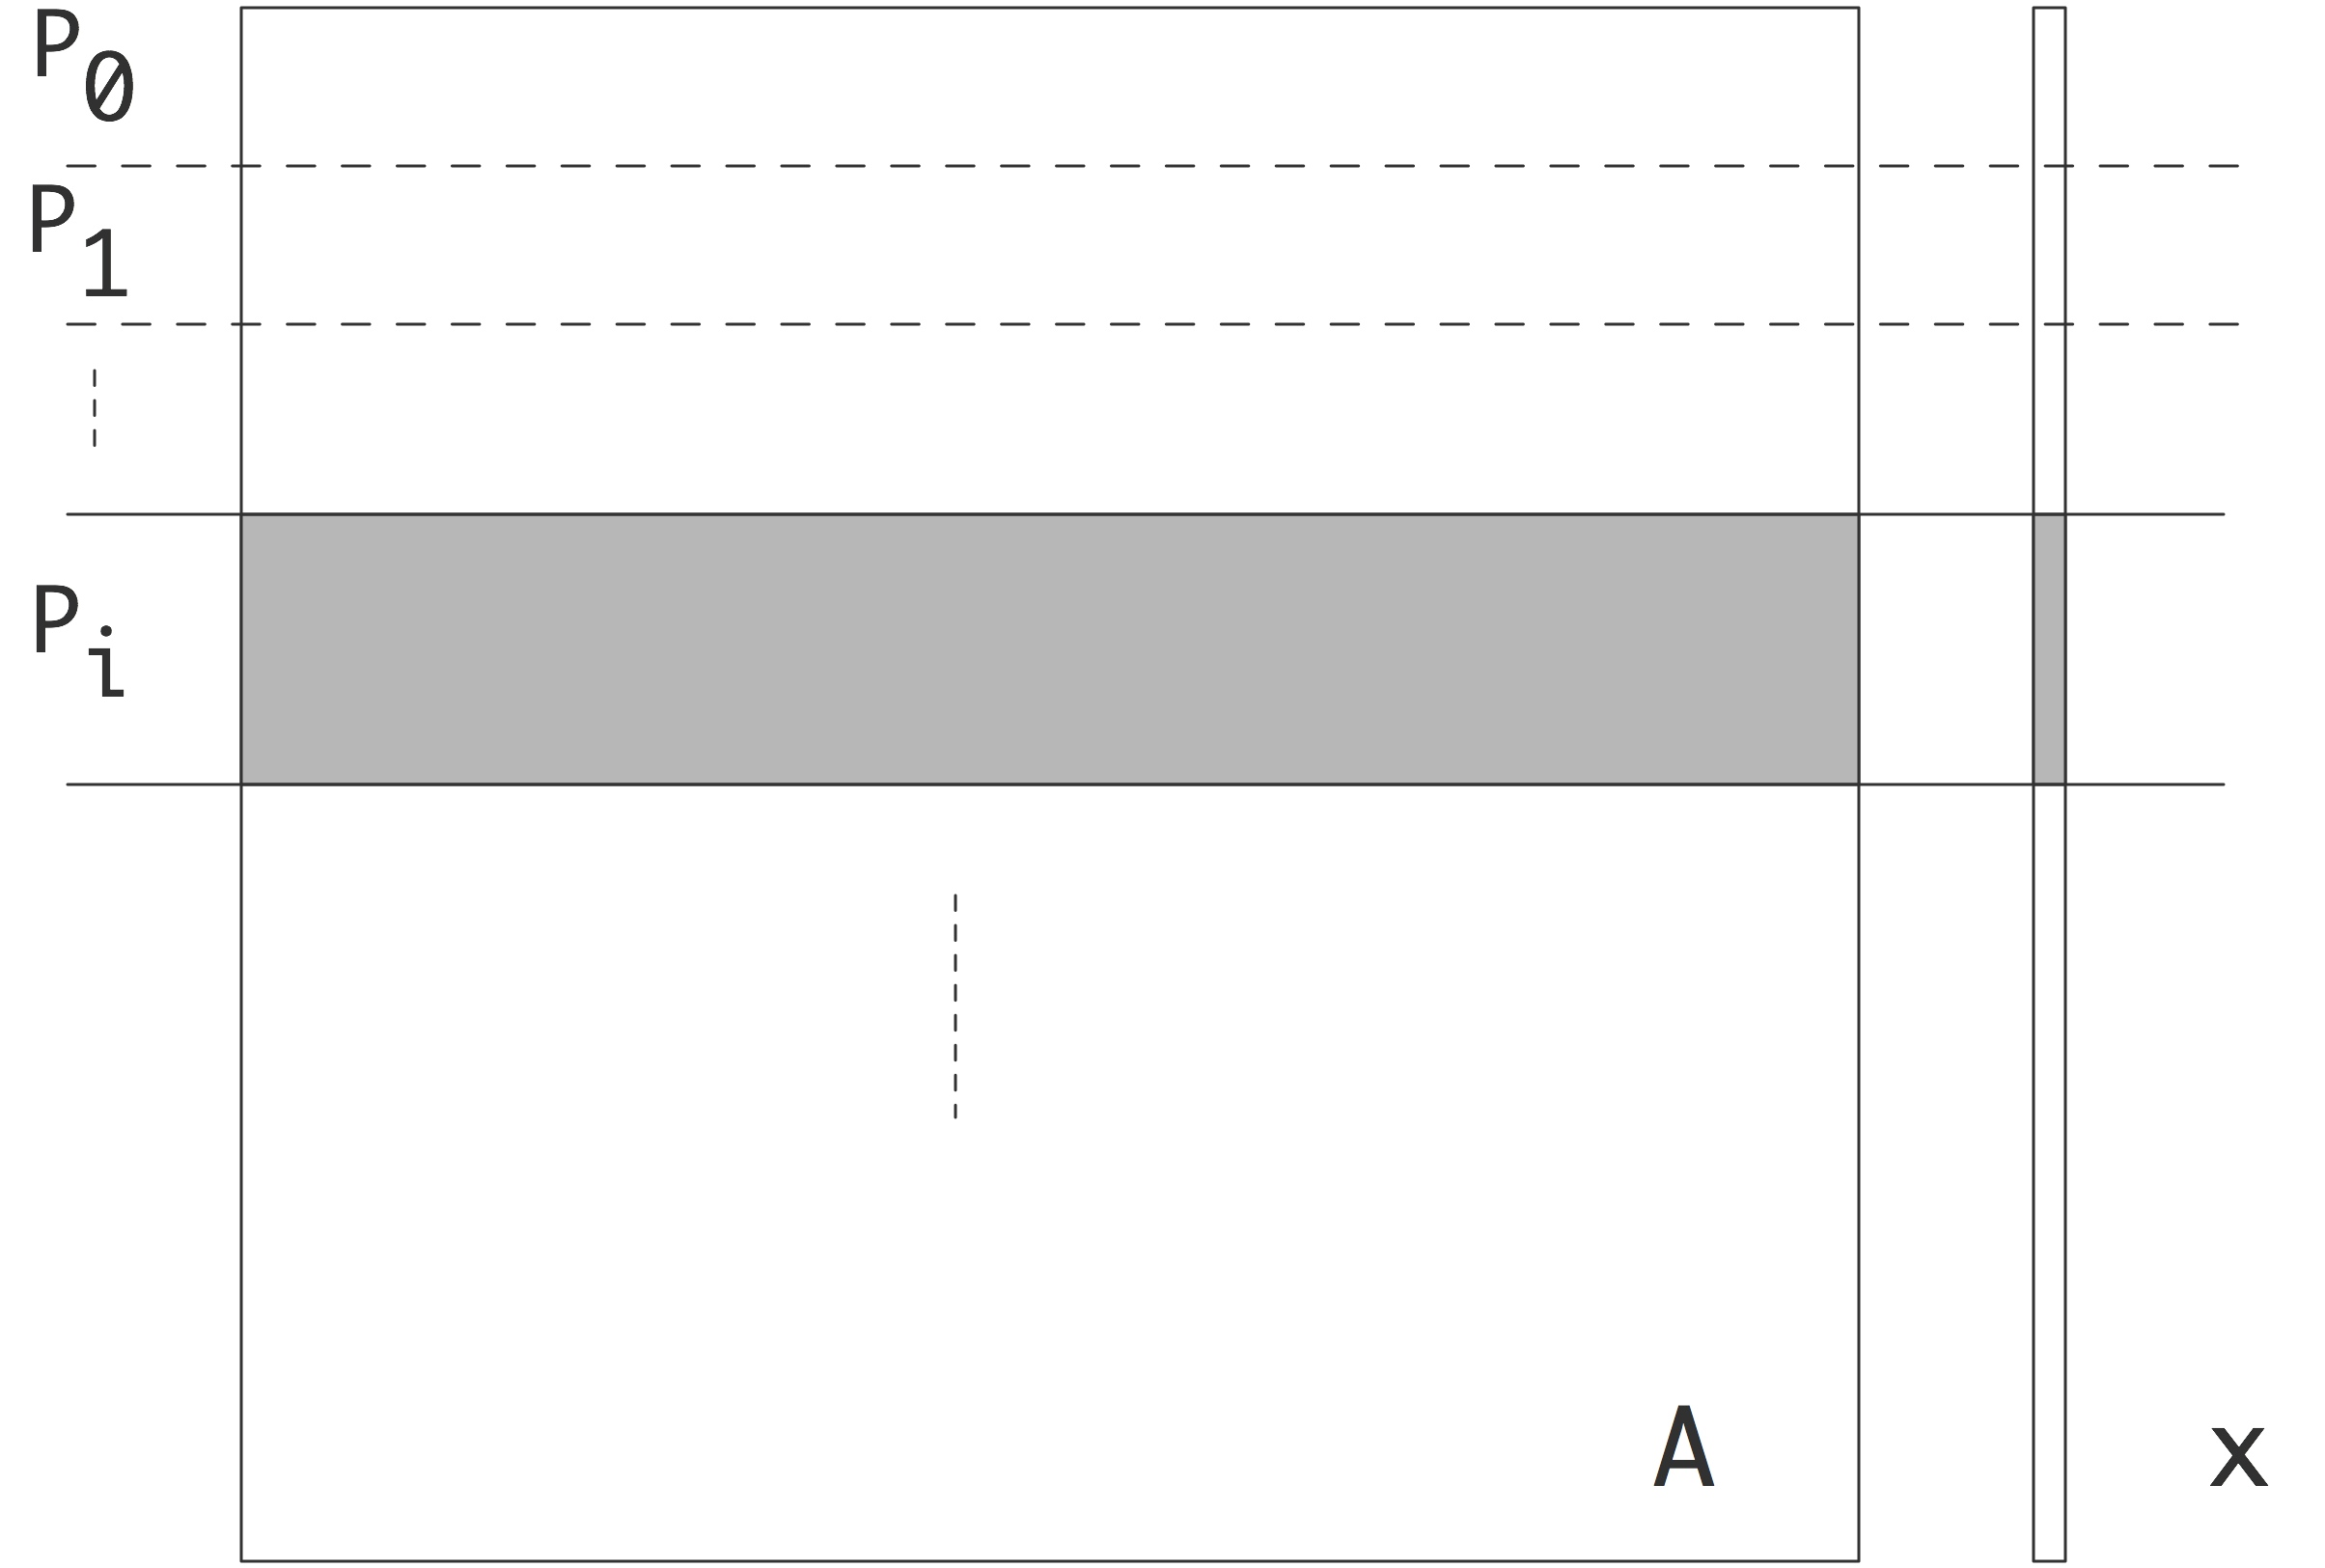
\includegraphics[scale=.12]{parallel-matrix}
  \caption{Matrix partitioning by block rows}
  \label{fig:parallel-matrix}
\end{figure}
%
In order for a matrix-vector product to be executable, both the input
and output vector need to be partitioned conforming to the matrix.

While for dense matrices the block row scheme is not scalable, for
matrices from \acp{PDE} it makes sense. There, a subdivision by matrix
blocks would lead to many empty blocks.

Just as with vectors, there is a local and global size; except that
that now applies to rows and columns.
Set sizes with
\indexpetscref{MatSetSizes}
and subsequently query them with
\indexpetscref{MatSizes}.
The concept of local column size is tricky:
since a process stores a full block row you may expect the local column size
to be the full matrix size, but that is not true.
The exact definition will be discussed later, but for square matrices it is a safe
strategy to let the local row and column size to be equal.

Instead of querying a matrix size and creating vectors accordingly,
the routine \indexpetscref{MatCreateVecs} can be used.
(Sometimes this is even required; see section~\ref{sec:petscfft}.)

\Level 1 {Nonzero structure}

In case of a dense matrix, once you have specified the size and the
number of MPI processes, it is simple to determine how much space PETSc
needs to allocate for the matrix. For a sparse matrix this is more
complicated, since the matrix can be anywhere between completely empty
and completely filled in. It would be possible to have a dynamic
approach where, as elements are specified, the space grows; however,
repeated allocations and re-allocations are inefficient. For this
reason PETSc puts a small burden on the programmer: you need to
specify a bound on how many elements the matrix will contain.

We explain this by looking at some cases. First we consider a matrix
that only lives on a single process. You would then use
\indexpetscref{MatSeqAIJSetPreallocation}.  In
the case of a tridiagonal matrix you would specify that each row has
three elements:
%
\begin{lstlisting}
MatSeqAIJSetPreallocation(A,3, NULL);
\end{lstlisting}

If the matrix is less regular you can use the third argument to give
an array of explicit row lengths:
\begin{lstlisting}
int *rowlengths;
// allocate, and then:
for (int row=0; row<nrows; row++)
  rowlengths[row] = // calculation of row length
MatSeqAIJSetPreallocation(A,NULL,rowlengths);
\end{lstlisting}

In case of a distributed matrix you need to specify this bound with
respect to the block structure of the matrix. As illustrated in figure~\ref{fig:petscmat},
a~matrix has a diagonal part and an off-diagonal part.
%
\begin{figure}[ht]
  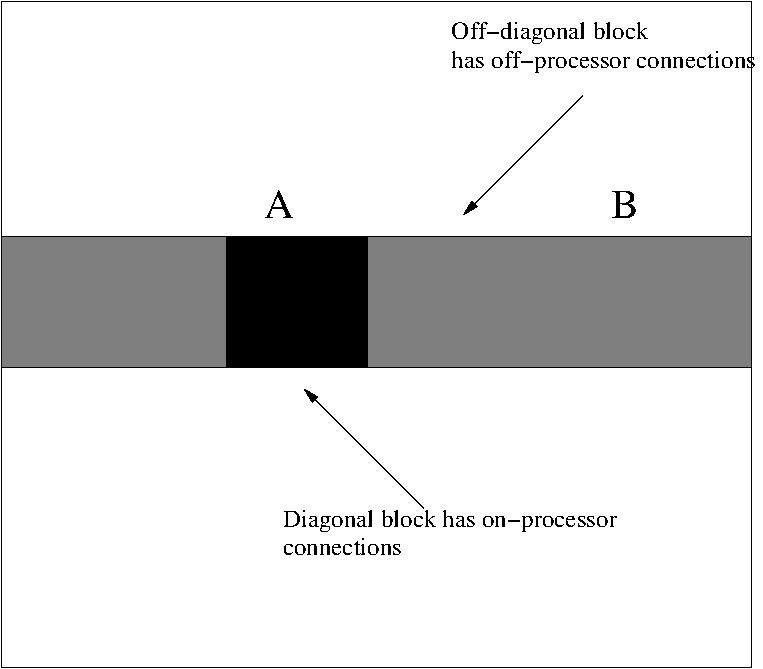
\includegraphics[scale=.5]{petscmat}
  \caption{The diagonal and off-diagonal parts of a matrix}
  \label{fig:petscmat}
\end{figure}
%
The diagonal part describes the matrix elements that couple elements of the
input and output vector that live on this process. The off-diagonal part contains the
matrix elements that are multiplied with elements not on this process, in order to compute
elements that do live on this process.

The preallocation specification now has separate parameters for
these diagonal and off-diagonal parts:
with 
\indexpetscxref{MatMPIAIJSetPreallocation}{MatSeqAIJSetPreallocation}.
you specify for both either a global upper bound on the number of nonzeros,
or a detailed listing of row lengths.
For the matrix of the \indexterm{Laplace equation}, this specification
would seem to be:
\begin{lstlisting}
MatMPIAIJSetPreallocation(A, 3, NULL, 2, NULL);
\end{lstlisting}
However, this is only correct if the block structure from the parallel division
equals that from the lines in the domain.
In general it may be necessary to use values that are an overestimate.
It is then possible to contract the storage by copying the matrix.

Specifying bounds on the number of nonzeros is often enough, and not too wasteful. However,
if many rows have fewer nonzeros than these bounds, a lot of space is
wasted. In that case you can replace the NULL arguments by an array
that lists for each row the number of nonzeros in that row.

\Level 1 {Matrix elements}
\label{sec:petsc-matset}

You can set a single matrix element with
%
\indexpetscref{MatSetValue}
%
or a block of them, where you
supply a set of $i$~and~$j$ indices, using
%
\indexpetscshow{MatSetValues}. 

After setting matrix elements, the matrix needs to be assembled. This
is where PETSc moves matrix elements to the right processor, if they
were specified elsewhere. As with vectors this takes two calls:
%
\indexpetscref{MatAssemblyBegin}
and
\indexpetscxref{MatAssemblyEnd}{MatAssemblyBegin}
%
which can be used to achieve \indextermbus{latency}{hiding}.

Elements can either be inserted
(\indexpetscshow{INSERT_VALUES}) or added
(\indexpetscshow{ADD_VALUES}).
You can not immediately mix these modes; to do so you need to call
\indexpetscshow{MatAssemblyBegin}~/ \indexpetscshow{MatAssemblyEnd}
with a value of \indexpetscdef{MAT_FLUSH_ASSEMBLY}.

PETSc sparse matrices are very flexible: you can create them empty and
then start adding elements. However, this is very inefficient in
execution since the \ac{OS} needs to reallocate the matrix every time
it grows a little. Therefore, PETSc has calls for the user to indicate
how many elements the matrix will ultimately contain.
%
\begin{lstlisting}
MatSetOption(A, MAT_NEW_NONZERO_ALLOCATION_ERR, PETSC_FALSE)
\end{lstlisting}

\Level 2 {Element access}

If you absolutely need access to the matrix elements, there are
routines such as 
\indexpetscref{MatGetRow}.
With this, any process can request, using global row numbering,
the contents of a row that it owns.
(Requesting elements that are not local requires the
different mechanism of taking submatrices; section~\ref{sec:petsc-submat}.)

Since PETSc is geared towards
\emph{sparse matrices}\index{matrix!sparse},
this returns not only the element values, but also the column numbers,
as well as the mere number of stored columns.
If any of these three return values are not needed, they can be
unrequested by setting the parameter passed to \clstinline{NULL}.

PETSc insists that you properly release the row again with
\indexpetscxref{MatRestoreRow}{MatGetRow}.

It is also possible to retrieve the full \ac{CRS} contents
of the local matrix with
\indexpetscshow{MatDenseGetArray},
\indexpetscshow{MatDenseRestoreArray},
\indexpetscshow{MatSeqAIJGetArray},
\indexpetscshow{MatSeqAIJRestoreArray}.
(Routines \indexpetscdepr{MatGetArray}~/ \indexpetscdepr{MatRestoreArray}
are deprecated.)

\Level 1 {Matrix viewers}

Matrices can be `viewed'
(see section~\ref{sec:petsc-view} for a discussion of the \indexpetscshow{PetscViewer} mechanism)
in a variety of ways, starting with the \indexpetscshow{MatView} call.
However, often it is more convenient to use online options such as
\begin{verbatim}
yourprogram -mat_view
yourprogram -mat_view draw
yourprogram -ksp_mat_view draw
\end{verbatim}
where \indexpetscoption{mat_view} is activated by the assembly routine,
while \indexpetscoption{ksp_mat_view} shows only the matrix used as
operator for a \indexpetscshow{KSP} object.
Without further option refinements this will display
the matrix elements inside the sparsity pattern.
Using a sub-option \n{draw} will cause the sparsity pattern to be
displayed in an \indexterm{X11} window.

\Level 1 {Matrix operations}

\Level 2 {Matrix-vector operations}

In the typical application of PETSc, solving large sparse linear
systems of equations with iterative methods, matrix-vector operations
are most important. Foremost there is the matrix-vector product
\indexpetscref{MatMult} and the transpose product
\indexpetscxref{MatMultTranspose}{MatMult}.
(In the complex case, the transpose product is not the Hermitian
matrix product; for that use \indexpetscshow{MatMultHermitianTranspose}.)

For the \ac{BLAS} \indextermtt{gemv} semantics
$y\leftarrow \alpha Ax + \beta y$,
\indexpetscref{MatMultAdd} computes
$z\leftarrow Ax +y $.

\Level 2 {Matrix-matrix operations}

There is a number of matrix-matrix routines such as
\indexpetscdef{MatMatMult}.

\Level 1 {Submatrices}
\label{sec:petsc-submat}

Given a parallel matrix, there are two routines for extracting submatrices:
\begin{itemize}
\item \indexpetscdef{MatCreateSubMatrix} creates a single parallel
  submatrix.
\item \indexpetscdef{MatCreateSubMatrices} creates a sequential
  submatrix on each process.
\end{itemize}

\Level 1 {Shell matrices}
\label{sec:mat-shell}

In many scientific applications, a matrix stands for some operator,
and we are not intrinsically interested in the matrix elements, but
only in the action of the matrix on a vector. In fact, under certain
circumstances it is more convenient to implement a routine that
computes the matrix action than to construct the matrix explicitly.

Maybe surprisingly, solving a linear system of equations can be
handled this way. The reason is that PETSc's iterative solvers
(section~\ref{sec:petsc-ksp}) only need the matrix-times-vector (and perhaps
the matrix-transpose-times-vector) product.

PETSc supports this mode of working. The routine \indexpetscref{MatCreateShell}
declares the argument to be a matrix given in operator form.

\Level 2 {Shell operations}

The next step is then to add the custom multiplication routine, which
will be invoked by \indexpetscshow{MatMult}:
%
\indexpetscref{MatShellSetOperation}

The routine that implements the actual product should have the same
signature as \indexpetscshow{MatMult}, accepting a matrix and two
vectors. The key to realizing your own product routine lies in the
`context' argument to the create routine. With
\indexpetscref{MatShellSetContext} you pass a pointer to some
structure that contains all contextual information you need. In your
multiplication routine you then retrieve this with \indexpetscref{MatShellGetContext}.

What operation is specified is determined by a keyword \lstinline+MATOP_<OP>+
where \lstinline{OP} is the name of the matrix routine, minus the \lstinline{Mat} part,
in all caps.

\begin{lstlisting}
MatCreate(comm,&A);
MatSetSizes(A,localsize,localsize,matrix_size,matrix_size);
MatSetType(A,MATSHELL);
MatSetFromOptions(A);
MatShellSetOperation(A,MATOP_MULT,(void*)&mymatmult);
MatShellSetContext(A,(void*)Diag);
MatSetUp(A);
\end{lstlisting}
(The call to \lstinline{MatSetSizes} needs to come before \lstinline{MatSetType}.)

\Level 2 {Shell context}

Setting the context means passing a pointer (really: an address) to
some allocated structure
\begin{lstlisting}
struct matrix_data mystruct;
MatShellSetContext( A, &mystruct );
\end{lstlisting}

The routine signature
has this argument as a \clstinline{void*} but it's not necessary to
cast it to that. Getting the context means that a pointer to your
structure needs to be set
\begin{lstlisting}
struct matrix_data *mystruct;
MatShellGetContext( A, &mystruct );
\end{lstlisting}
Somewhat confusingly, the Get routine also has a \clstinline{void*}
argument, even though it's really a pointer variable.

\Level 1 {Multi-component matrices}
\label{sec:matfieldsplit}

For multi-component physics problems there are essentially
two ways of storing the linear system
\begin{enumerate}
\item Grouping the physics equations together, or
\item grouping the domain nodes together.
\end{enumerate}
In both cases this corresponds to a block matrix, but
for a problem of $N$ nodes and $3$ equations, the
respective structures are:
\begin{enumerate}
\item $3\times 3 $ blocks of size~$N$, versus
\item $N\times N$~blocks of size~$3$.
\end{enumerate}
The first case can be pictured as
\[ 
\begin{pmatrix}
  A_{00}&A_{01}&A_{02}\\ A_{10}&A_{11}&A_{12}\\ A_{20}&A_{21}&A_{22}\\ 
\end{pmatrix}
\]
and while it looks natural, there is a computational problem with it.
Preconditioners for such problems often look like
\[ 
\begin{pmatrix}
  A_{00}&\\ &A_{11}&\\ &&A_{22}\\ 
\end{pmatrix}
\quad\hbox{or}\quad
\begin{pmatrix}
  A_{00}&&\\ A_{10}&A_{11}&\\ A_{20}&A_{21}&A_{22}\\ 
\end{pmatrix}
\]
With the block-row partitioning of PETSc's matrices, this means
at most a 50\% efficiency for the preconditioner solve.

It is better to use the second scheme, which requires the
\indexpetscdef{MATMPIBIJ} format,
and use so-called \indextermsub{field-split}{preconditioner}s;
see section~\ref{sec:pcfieldsplit}.

\Level 1 {Fourier transform}
\label{sec:petscfft}

The \indexac{FFT} can be considered a matrix-vector multiplication.
PETSc supports this by letting you create a matrix with \indexpetscdef{MatCreateFFT}.
This requires that you add an FFT library, such as \indexterm{fftw},
at configuration time; see section~\ref{sec:petsc-external}.

FFT libraries may use padding, so vectors should be created with
\indexpetscdef{MatCreateVecsFFTW},
not with an independent \indexpetscshow{VecSetSizes}.

The \indexterm{fftw} library does not scale the output vector,
so a forward followed by a backward pass gives a result that is too large
by the vector size.

\cverbatimsnippet[examples/petsc/c/fftsine.c]{vecviewbeforeafter}

\begin{multicols}{2}
One full cosine wave:
\begin{verbatim}
1.
0.809017 + 0.587785 i
0.309017 + 0.951057 i
-0.309017 + 0.951057 i
-0.809017 + 0.587785 i
-1. + 1.22465e-16 i
-0.809017 - 0.587785 i
-0.309017 - 0.951057 i
0.309017 - 0.951057 i
0.809017 - 0.587785 i
\end{verbatim}
\columnbreak
Frequency $n=1$ amplitude~$\equiv1$:
\begin{verbatim}
-2.22045e-17 + 2.33487e-17 i
1. - 9.23587e-17 i
2.85226e-17 + 1.56772e-17 i
-4.44089e-17 + 1.75641e-17 i
-3.35828e-19 + 3.26458e-18 i
0. - 1.22465e-17 i
-1.33873e-17 + 3.26458e-18 i
-4.44089e-17 + 7.59366e-18 i
7.40494e-18 + 1.56772e-17 i
0. + 1.8215e-17 i
\end{verbatim}
\end{multicols}

Strangely enough, the backward pass does not need to be scaled:

\cverbatimsnippet[examples/petsc/c/fftsine.c]{fftaccuracy}

\Level 0 {Index sets and Vector Scatters}

In the \ac{PDE} type of applications that PETSc was originally intended for,
vector data can only be real or complex: there are no vector of integers.
On the other hand, integers are used for indexing into vector,
for instance for gathering boundary elements into a \indexterm{halo region},
or for doing the \indextermsub{data}{transpose} of an \indexac{FFT} operation.

To support this, PETSc has the following object types:
\begin{itemize}
\item An \clstinline{IS} object describes a set of integer indices;
\item a \clstinline{VecScatter} object describes the correspondence between
  a group of indices in an input vector and a group of indices in an output vector.
\end{itemize}

\Level 1 {IS: index sets}
\label{sec:petsc-is}

An \clstinline{IS} object contains a set of \indexpetscshow{PetscInt} values.
It can be created with
\begin{itemize}
\item \indexpetscdef{ISCreate} for creating an empty set;
\item \indexpetscdef{ISCreateStride} for a strided set;
\item \indexpetscdef{ISCreateBlock} for a set of contiguous blocks,
  placed at an explicitly given list of starting indices.
\item \indexpetscshow{ISCreateGeneral} for an explicitly given list of indices.
\end{itemize}

For example, to describe odd and even indices (on two processes):
%
\cverbatimsnippet[examples/petsc/c/oddeven.c]{isoddeven}

After this, there are various query and set operations on index sets.

You can read out the indices of a set by \indexpetscdef{ISGetIndices}
and \indexpetscdef{ISRestoreIndices}.

\Level 1 {VecScatter: all-to-all operations}
\label{sec:petsc-vs}

A \indexpetscdef{VecScatter} object is a generalization of an
all-to-all operation. However, unlike MPI \indexmpishow{MPI_Alltoall},
which formulates everything in terms of local buffers, a
\clstinline{VecScatter} is more implicit in only describing indices in
the input and output vectors.

The \indexpetscref{VecScatterCreate} call has as arguments:
\begin{itemize}
\item An input vector. From this, the parallel layout is used; any
  vector being scattered from should have this same layout.
\item An \clstinline{IS} object describing what indices are being
  scattered; if the whole vector is rearranged, \clstinline{NULL}
  (Fortran: \indexpetsctt{PETSC_NULL_IS}) can be given.
\item An output vector. From this, the parallel layout is used; any
  vector being scattered into should have this same layout.
\item An \clstinline{IS} object describing what indices are being
  scattered into; if the whole vector is a target, \clstinline{NULL} can
  be given.
\end{itemize}

As a simple example, the odd/even sets defined above can be used to
move all components with even index to process zero, and the ones with
odd index to process one:
%
\cverbatimsnippet[examples/petsc/c/oddeven.c]{vsoddeven}

Note that the index set is applied to the input vector, since it
describes the components to be moved. The output vector uses
\clstinline{NULL} since these components are placed in sequence.

\begin{exercise}
  Modify this example so that the components are still separated
  odd/even, but now placed in descending order on each process.
\end{exercise}

\begin{exercise}
  Can you extend this example so that process~$p$ receives
  all indices that are multiples of~$p$? Is your solution correct if
  \clstinline{Nglobal} is not a multiple of \clstinline{nprocs}?
\end{exercise}

\Level 2 {More VecScatter modes}

There is an added complication, in that a \clstinline{VecScatter} can
have both sequential and parallel input or output vectors.
Scattering onto process zero is also a popular option.

\Level 0 {AO: Application Orderings}

PETSc's decision to partition a matrix by contiguous block rows
may be a limitation in the sense an application can have a natural
ordering that is different. For such cases the \indexpetscdef{AO} type
can translate between the two schemes.

\Level 0 {Partitionings}

By default, PETSc uses partitioning of matrices and vectors based on
consecutive blocks of variables.
In regular cases that is not a bad strategy.
However, for some matrices a permutation and re-division can
be advantageous.
For instance, one could look at the \indextermbus{adjacency}{graph},
and minimize the number of \indextermbus{edge}{cuts}
or the sum of the \indextermbus{edge}{weight}s.

This functionality is not built into PETSc, but can be provided by
\emph{graph partitioning packages}\index{graph!partitioning!packages}
such as \indexterm{ParMetis} or \indexterm{Zoltan}.
The basic object is the \indexpetscdef{MatPartitioning},
with routines for 
\begin{itemize}
\item Create and destroy: \indexpetscdef{MatPartitioningCreate},
  \indexpetscdef{MatPartitioningDestroy};
\item Setting the type \indexpetscdef{MatPartitioningSetType}
  to an explicit partitioner, or something generated
  as the dual or a refinement of the current matrix;
\item Apply with \indexpetscdef{MatPartitioningApply},
  giving a distribued \indexpetscshow{IS} object,
  which can then be used in \indexpetscshow{MatCreateSubMatrix}
  to repartition.
\end{itemize}
Illustrative example:
\begin{lstlisting}
MatPartitioning part;
MatPartitioningCreate(comm,&part);
MatPartitioningSetType(part,MATPARTITIONINGPARMETIS);
MatPartitioningApply(part,&is);
/* get new global number of each old global number */
ISPartitioningToNumbering(is,&isn);
ISBuildTwoSided(is,NULL,&isrows);
MatCreateSubMatrix(A,isrows,isrows,MAT_INITIAL_MATRIX,&perA);
\end{lstlisting}

Other scenario:
\begin{lstlisting}
MatPartitioningSetAdjacency(part,A);
MatPartitioningSetType(part,MATPARTITIONINGHIERARCH);
MatPartitioningHierarchicalSetNcoarseparts(part,2);
MatPartitioningHierarchicalSetNfineparts(part,2);
\end{lstlisting}
